\subsection{Überblick}
Man hat sich bei allink bis heute noch nicht richtig mit dem eigenen Organigramm
auseinander gesetzt. Zur Zeit existiert nur die Unterscheidung zwischen Mitarbeitern 
und Partnern, aus denen sich gleichzeitig die Geschäftsleitung zusammen setzt.

\begin{figure}[htbp]
\begin{center}
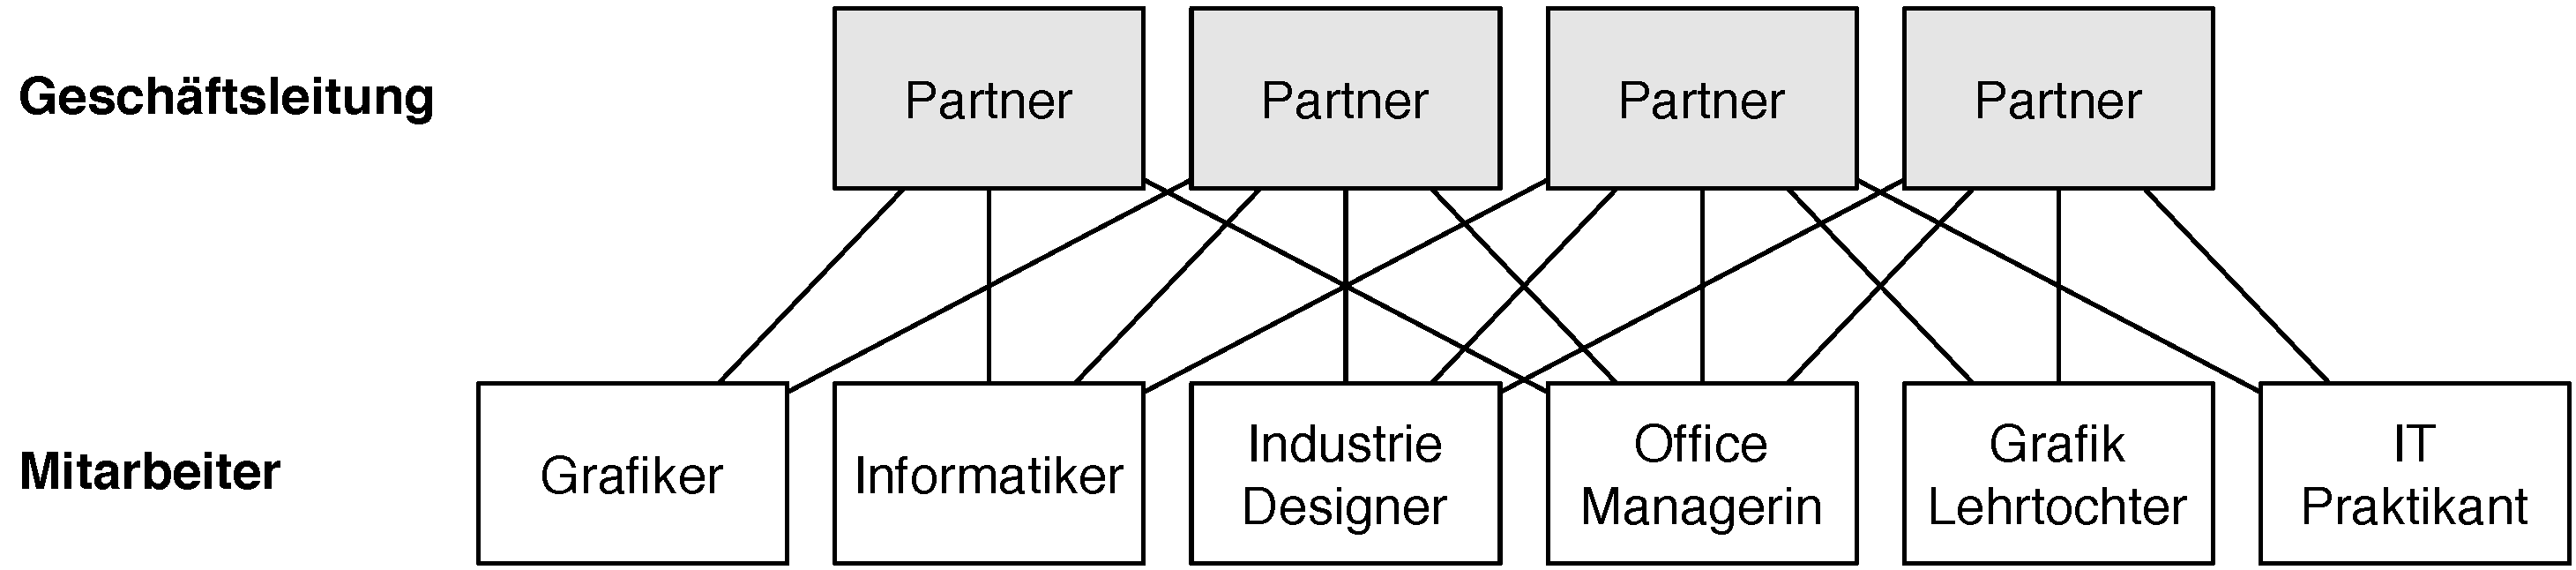
\includegraphics[width=0.95\textwidth,angle=0]{./bilder/ist_organigramm.pdf}
\caption{Aktuelles Organigramm von allink}
\label{pic:ist_organigramm}
\end{center}
\end{figure}

Die Partner kümmern sich um die Projekte, deren Leitung sie übernommen haben
und versuchen anhand den verfügbaren Mitarbeitern und Fachkräften die Projekte 
erfolgreich durchzuführen. Jeder Partner organisiert die benötigten Mitarbeiter
selbst. Dabei kann es vorkommen, dass ein Mitarbeiter parallel an
mehreren Projekten arbeiten muss.

Dies funktioniert so lange gut, bis die Mitarbeiter völlig ausgelastet oder sogar
überbelastet sind. Dies gilt natürlich auch für die Partner. Sobald ein gewisses 
Auftragspensum erreicht ist, kommen die parallel laufenden Projekte ins Stocken 
und schwächen sich gegenseitig. Die Inexistenz eines Projektablaufes bringt
einige Probleme mit sich.

Die Ressourcenüberbelastung ist nur ein Problem, das zum Vorschein kommt. In der
Abbildung \ref{pic:voruntersuchung_projektablauf} verschaffe ich mir einen 
Überblick über die möglichen Gefahren und Schwächen des aktuellen Projektablaufes.

\begin{figure}[htbp]
\begin{center}
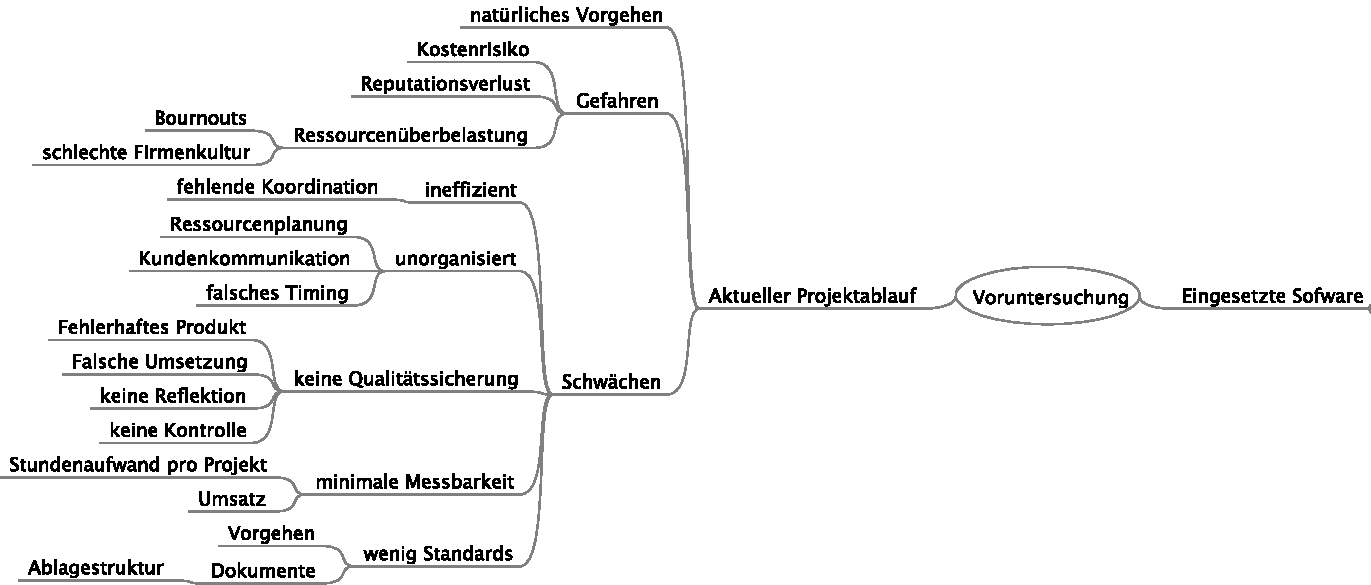
\includegraphics[width=0.95\textwidth,angle=0]{./mindmaps/voruntersuchung_projektablauf.pdf}
\caption{MindMap Voruntersuchung des aktuellen Projektablaufes}
\label{pic:voruntersuchung_projektablauf}
\end{center}
\end{figure}

\subsubsection{Wenig Standards}
Man hält vor, während und nach einem Projekt nur an wenige Standards fest. 
Das ganze Vorgehen ist nicht einheitlich, da in jedem Projekt wieder von
neuem entschieden wird, wie man vorgehen will. Es werden nur wenige einheitlichen
Dokumente verwendet, zum Beispiel für die Erstellung von Offerten und Rechnungen.
Aber auch da entstehen schnell Fehler, z.B. während der Umstellungen des 
Mehrwert Steuersatzes von 7.6\% auf 8\%. Da kein einheitliches Basistemplate
existiert, muss jeder der eine Rechnung schreibt noch einmal sicherstellen, ob
auch der korrekte Steuersatz hinterlegt ist. 

\subsubsection{Unorganisiert}
Durch die Überbelastung können mit der Zeit die versprochenen Timings
nicht mehr eingehalten werden. Da die Ablagestrukturen nicht einheitlich geregelt
sind, kann es vorkommen, dass ein Mitarbeiter einem Kunden ein veraltetes oder
noch nicht freigegebenes Dokument sendet. Dies zieht einen zusätzlichen 
Mehraufwand mit sich, da man sich beim Kunden entschuldigen und rechtfertigen
muss. Zusätzlich strapaziert es auch die Beziehung zum Kunden.

\subsubsection{Ineffizient}
Einfache Abläufe werden so unnötig verkompliziert und aufgehalten. Die ganze
Struktur wird langsam und ineffizient. Was sich wiederum negativ auf die zur
Verfügung stehende Zeit auswirkt.

\subsubsection{Keine Qualitätssicherung}
Oft bleibt gegen Ende eines Projektes dann zu wenig Zeit die nötige 
Qualitätskontrollen durchzuführen, da man sich möglichst schnell um ein anderes,
möglicherweise auch schon überfälliges, Projekt kümmern muss. Der Kunde entdeckt
dann offensichtliche Fehler selbst und zweifelt zwangsläufig an der ganzen Arbeit.

\subsubsection{Minimale Messbarkeit}
Auch bietet die fehlende bzw. chaotische Struktur nur wenige Punkte um Kennzahlen
zu messen. Den Umsatz den man mit dem Projekt erzielt hat ist zwar bekannt,
jedoch kann nur aus dem Gefühl heraus erahnt werden, ob mit dem Projekt einen
Gewinn für die Firma erzielt werden konnte. Die Mitarbeiter sind zwar angehalten
ihre Stunden in ein gemeinsames Stundelog pro Projekt einzutragen, jedoch werden
die Informationen nicht ausgewertet und können nicht mehr einzelnen Mitarbeitern
zugeordnet werden.

\subsubsection{Kostenrisiko}
Durch die fehlende Kontrolle während eines Projektes, verliert man die
Übersicht über die Aufwände und schlussendlich die Kosten. Dadurch entsteht
ein Kostenrisiko, welches Konsequenzen für die Liquidität von allink haben könnte.

\subsubsection{Ressourcenüberbelastung}
Die Belastung für den Mitarbeiter wie auch für die Partner ist so über
längere Zeit nicht tragbar. Durch eine Überarbeitung kann es zu Ausfällen kommen, die
die Situation zusätzlich verschlimmern könnten. Das ganze Endet in einer 
schlechten Firmenkultur und das Unternehmung beginnt von innen zu zerfallen.

\subsubsection{Reputationsverlust}
Da man Timings nicht mehr einhalten kann und man sich gegenüber dem Kunden
oft rechtfertigen muss entsteht ein schlechtes Bild der Unternehmung und sie
verliert an Vertrauen. Da die Konkurrenz im Tätigkeitsfeld der allink relativ
gross ist, ist ein möglicher Absprung und Angenturwechsel seitens des Kunden nicht 
auszuschliessen.

\subsection{Zurzeit eingesetzte Software}
Bei der Untersuchung der zur Zeit eingesetzten Sofware beschränke ich mich auf jene,
die einen direkten Einfluss auf den aktuellen Projektablauf bei allink haben.
Ich liste keine Software auf, die zur Erbringung der eigentlichen Dienstleistungen
von allink eingesetzt werden.

\begin{figure}[htbp]
\begin{center}
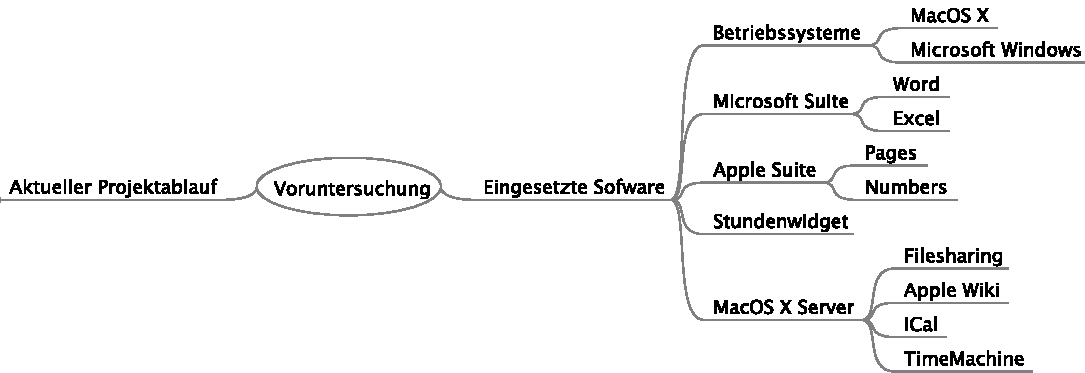
\includegraphics[width=0.95\textwidth,angle=0]{./mindmaps/voruntersuchung_software.pdf}
\caption{MindMap Voruntersuchung der eingesetzten Software}
\label{pic:voruntersuchung_software}
\end{center}
\end{figure}

\subsubsection{Betriebssysteme}
Als Hauptbetriebssystem verwendet allink Mac OS X\footnote{Betriebssystem von Apple, \url{http://www.apple.com/macosx/}}.
Es läuft auf allen Arbeitsstationen der Mitarbeiter und Partner. Zusätzlich haben einige der
Entwickler noch Microsoft Windows\footnote{Betriebssystem von Microsof, \url{http://www.microsoft.com/windows/}}
über eine Virtualisierungslösung installiert. Dies wird zu Testzwecken benötigt.

\subsubsection{Microsoft Suite}
Da viele Kunden mit Microsoft Produkten arbeiten benötigt auch allink die
Office Suite\footnote{Microsoft Office für Mac, \url{http://www.microsoft.com/germany/mac}}, 
um Dateien mit Kunden ohne Interoperabilitätsprobleme
austauschen zu können. Nicht jede Arbeitsstation verfügt zur Zeit über eine
Installation.

\subsubsection{Apple Suite}
Für interne Zwecke setzt allink zur Zeit auf die Apple eigene Office Suite
iWork\footnote{Office Suite von Apple, \url{http://www.apple.com/de/iwork/}}.
Pages wird zur Erstellung von Offerten und Rechnungen verwendet. Mit Numbers
werden Tabellenkalkulationen wie die Liquiditätsplanung oder Lohnblätter erstellt.
Da dies aber lange nicht so von der Geschäftsleitung kommuniziert wurde, existieren
auch einige Excel Files, das Pendant der Microsoft Office Suite.

\subsubsection{Stundenwidget}
Das Stundenwidget ist eine selbst geschriebene Software von allink und läuft
im Dashboard\footnote{Widget Lösung von Apple, \url{http://www.apple.com/downloads/dashboard/}} des Betriebssystems.
Es ermöglicht Stunden auf ein Projekt zu buchen, wie man auf dem Screenshot \ref{pic:ist_widget}
sehen kann.

\begin{figure}[htbp]
\begin{center}
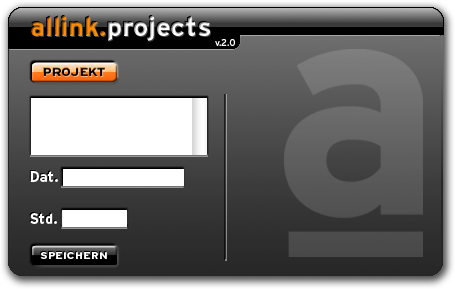
\includegraphics[width=0.55\textwidth,angle=0]{./bilder/ist_widget.png}
\caption{Aktuelles Stundenwidget von allink}
\label{pic:ist_widget}
\end{center}
\end{figure}

Die Daten werden auf dem
eigenen Server gespeichert und pro Projekt abgelegt. Dieses Widget ist auf allen
Arbeitsstationen installiert und wird von den Mitarbeitern gelegentlich verwendet
um ihre Stunden auf ein Projekt zu rapportieren.

\subsubsection{MacOS X Server}
Auf dem Server liegt das zentrale Dateiablagesystem. Die Zugriffsrechte können
auf dem Server für jede Freigabe definiert werden. So haben zum Beispiel
die Mitarbeiter keinen Zugriff auf den Administrationsordner der Geschäftsleitung.
Über diesen Server laufen auch die einzelnen Firmenkalender der Partner. Sie
können so gemeinsam Termine buchen und haben stets Einblick in die anderen
Kalender.
